\documentclass[12pt,a4paper]{article}

%\usepackage[german]{babel} %Für die indirekte Angabe von Umlauten. Es müssen dann Umlaute wie folgt im Code angegeben werden: "a "o "u "s.

\usepackage[utf8]{inputenc}
%dieses Paket ermöglicht uns, Umlaute im Text als solche eingeben zu können (Windows/Linux)

\usepackage{amsmath, amsthm, amssymb}
\usepackage{enumerate}
\usepackage{graphicx}
\usepackage{lscape}
\usepackage{setspace}
\onehalfspacing
\usepackage{wrapfig}
\usepackage{hyperref}% für die Einbettung von Hyperlinks
\usepackage{multirow}
\usepackage[round]{natbib}
\usepackage{longtable}
\bibliographystyle{apalike}

\newtheorem{definition}{Definition}[section]
\newtheorem{interview}{Interview}[section]
\newtheorem{satz}{Satz}[section]
\newtheorem{beispiel}{Beispiel}[section]
\newtheorem{bemerkung}{Bemerkung}[section]
\newtheorem{literaturverzeichnis}{Literaturverzeichnis}[section]

\usepackage[top=20mm, bottom=20mm, left=20mm, right=20mm, includehead]{geometry} % Document Margins
\setlength{\topmargin}{0cm}
\setlength{\parindent}{0mm}
\setlength{\parskip}{2mm}
\setlength{\evensidemargin}{0mm}
\setlength{\oddsidemargin}{0cm}
%\pagestyle{headings}

\providecommand{\tightlist}{%
  \setlength{\itemsep}{0pt}\setlength{\parskip}{0pt}}

\begin{document}
\thispagestyle{empty}
\vspace*{-3cm}
\begin{center}
\large \textsc{}
\vspace{0.5cm}
%\hrule
\vspace{5.5cm}
{\large}\\
\vspace{1cm}
{\Large \bf
Aufgabendauern automatisch schätzen}\\
\vspace*{1cm}
{\large mit Aritmethik und Künstlicher Intelligenz}
\end{center}
\vspace*{14cm}


\hspace*{\fill} von Stefan Hoffmann und others, \today

\newpage
\pagenumbering{Roman}
\tableofcontents

%\newpage
%\addcontentsline{toc}{section}{tables} %wenn es im Inhaltsverzeichnis erscheinen soll - sonst auskommentieren mit "%"
%\listoftables

%\newpage
%\addcontentsline{toc}{section}{Abbildungsverzeichnis} %wenn es im Inhaltsverzeichnis erscheinen soll - sonst auskommentieren mit "%"
%\listoffigures

\newpage
\pagenumbering{arabic}
%Und nun kommen wir zur Arbeit und fangen an die Seiten mit Arabischen Zahlen zu zählen
\hypertarget{foreword}{%
\section{Vorwort}\label{foreword}}

Um es kurz zu machen: Aufgabendauern schätzen ist im Grunde eine Katastrophe. Man kann viel Aufwand hineinstecken und dennoch werden sie nie wirklich gut. Und während man nach Perfektion strebt und sich selbst dabei aufreibt investiert man mehr und mehr Zeit und erwischt sich letztlich dabei, dass man mehr Zeit mit schätzen verbraucht, als die Aufgabe eigentlich dauert und/oder wert ist.

Leider werden wir gleichzeitig Schätzungen nicht vollständig los, weil wirtschaftliches Handeln nun mal eine entsprechende Betrachtungsweise vor Beginn einer Arbeit voraussetzt. 

Wir können Sie nicht loswerden, aber mit passenden Automatisierungen können wir mehr positive Effekte und weniger negative Effekte gewinnen:

\begin{itemize}
\tightlist
\item
    Da wir die Schätzungen Algorithment überlassen und diese anhand tatsächlicher Daten vorgehen, sind sie nicht einfach nur "wildes Herumgerate". Sie können eine bestimmte Arbeits-Pipeline beobachten und besser und besser werden, je nachdem wie sich die Pipeline (z.B. unsere Abteilung) schlägt.
\item
  Algorithmen arbeiten systematisch. Wie sie zu ihrem Ergebnis gelangen ist dokumentiert. Auf diese Weise nehmen sie typische menschliche Fehler aus der Gleichung, z.B. : Der Chef wird die Schätzung eh halbieren, also verdoppel ich sie besser... Wenn der Chef die Schätzung sieht reduziert er sie auf 15 Minuten, weil die Komplexität der Herausforderung nicht einfach sichtbar ist. (... außerdem würde der Kunde diese Schätzung nie akzeptieren, weil ...)
\item
  Da Arbeiten wie dieses PDF und wissenschaftliche Methoden verfügbar sind, können Algorithmen auf ihre Wirksamkeit geprüft werden. Damit können sie systematisch verbessert werden. Damit haben wir die Möglichkeit besser und besser zu werden.
\item
  Man kann einfacher kommunizieren, dass es sich um eine Schätzung handelt. Während eigentlich alles darauf hin deutet, dass die Schätzung eh besser ist, als sie je ein Mensch machen könnte, ist es sogar klarer, dass Algorithmen eben nur so gut sind wie sie sein können. Es sind also wirklich wirklich Schätzungen und es ist kein Fixdatum, dass herausgegeben wird.
\item
  Geschäftsmenschen können ihre Zeitschätzungen in nahezu Echtzeit haben. (Natürlich werden sie früher oder später an den Texten herumbasteln, um zu gucken, wie die Algos funktionieren und wie sie sie zu günstigen Schätzungen beschupsen. Aber der daraus entstehende Schaden ist klar ihr eigener, also los Jungs, schneidet euch nicht am Papier. Außerdem ist es nicht unbedingt gesagt, dass das nicht aus Versehen tatsächlich funktioniert. Wenn z.B. die Änderung in 2 Anwendungen implementiert werden könnte, aber die eine ist nun mal einfacher zu erweitern, was die Daten so auch wiederspiegeln? Win-win)
\item
  Ein sehr wichtiger Punkt ist, dass die Entwickler jener Geschäftsmenschen in der Zeit programmieren können. Frei nach dem Motto: Wenn ich 40 Stunden pro Woche für Dich Projekte plane, warum bist Du am Ende der Woche entsetzt, wenn nichts programmiert ist? Automatisierung der Schätzungen bedeutet also wir Entwickler sind produktiver.
\item
  Der Umstand, dass wir Entwickler das machen können, was sie mehr mögen - Software entwickeln - macht uns glücklicher. Wir müssen uns nicht mehr um die Leute kümmern, die uns nach  Schätzungen fragen, nur um sie dann, wenn sie nicht von vornherein mies waren, ad absurdum zu führen um dann für nur mehr oder weniger scheinbar existente Deadlines zur Rechenschaft gezogen zu werden.
\end{itemize}

Also soweit die Idee. Schauen wir, ob es funktioniert. Vielleicht nicht, aber ich schätze die Chance eigentlich recht positiv ein. Schließlich ist das einzige, was wir zu verlieren haben, schlechte Schätzungen. Und das was wir gewinnen können sind Schätzungen, vielleicht genauso mies, aber wenigstens kosten sie uns keine Zeit mehr. Also los gehts.


\section{Begleitendes Material}

Mit diesem E-Book verbunden werden einige Dinge mit herausgegeben:


\subsection{EstimatePS}

EstimatePS ist ein Powershell-Modul zur Schätzung von Aufgaben auf der Kommandozeile. 
Es implementiert im Moment (17.10.2021) nur A001.
Der Code ist in diesem Repository enthalten, aber das Modul ist auch in der Powershell-Gallery verfügbar.

\begin{verbatim}
Install-Module EstimatePS
\end{verbatim}

Ein Beispiel zur Anwendung findest Du in diesem Repository hier unter Source\\EstimatePS-Example .

Möge es jenen helfen, die es brauchen.



\newpage{}

\section{Qualitätssicherung}

\subsection{Allgemein}

Wenn wir in den nächsten Kapiteln Algorithmen betrachten, dann müssen 
wir sagen können, wie gut sie sind. Und dazu müssen wir einen gemeinsamen Standard etablieren.

Die Ausführung der Algorithmen wird über die `Scripts/configuration.json` 
koordiniert. Hier können Datenquellen angegeben werden, unabhängig davon 
werden die Algorithmen konfiguriert, jeweils mit ihren Aufrufen für "Lernen"
und "Anwenden". 

Des Weiteren kann ein flexibler Parameter angegeben werden, falls für einen Algorithmus mehrere Varianten existieren. Die notwendigen Aufrufe werden dabei automatisch permutiert, so dass man sich darum nicht kümmern muss. Die Dateinamen, in denen das Modell für den entsprechenden Algorithmus abgelegt wird, wird ebenfalls automatisch zusammengebaut.

Datenquellen werden in einer Kombination angegeben. Jeweils eine Datenquelle für das Erlernen und eine für den Test. 

\subsection{Aufbau der Eingabedatenquellen}

Wir arbeiten im Rahmen dieser Arbeit ausschließlich mit CSV als Dateiformat. 

\begin{itemize}
  \item Wir trennen Werte mit dem Komma.
  \item Wir umschließen Werte mit Double-Quotes.
  \item Zahlen werden mit Punkt (.) als Dezimaltrennzeichen angegeben, also z.B. 10.36 .
  \item Das Umschließen der Zahlen ebenfalls mit Double-Quotes ist erlaubt.
  \item In der ersten Zeile stehen die Spaltennamen.
\end{itemize}

Wir nutzen folgende Spalten:
\begin{itemize}
  \item Spalte 1: "Name" (Zeichenkette)
  \item Spalte 2: "Time spent" (Fließkommazahl)\\
        Die "Time spent" wird in Stunden angegeben.   
\end{itemize}

In unseren Testdaten ist die Genauigkeit auf 3 Nachkommastellen begrenzt, 
es sollten aber ohne Probleme noch mehr verwendet werde können.

Es können weitere Spalten angegeben werden, falls sie vom Algorithmus verwendet werden sollen. In dieser Arbeit verwenden wir aber nur diese beiden. 

\subsection{Aufbau der Ausgabedatenquellen}

Durch die Verarbeitung über einen Algorithmus werden im Verzeichnis Scripts\\output Ausgabe-CSV-Dateien erstellt. Das sind im Grunde die gleichen Dateien mit folgenden zusätzlichen Spalten:

\begin{itemize}
  \item Spalte "DurationInSeconds"\\ 
        "Time spent" umgerechnet in Sekunden.
  \item Spalte "EstimateInSeconds"\\ 
        Die Dauer, die der Algorithmus geschätzt hat, ebenfalls in Sekunden.
\end{itemize}

\subsection{Tabellarische Analyse}

Am Ende des E-Books wird eine Tabelle mit den Ergebnissen aller Algorithmen über alle Datenmengen-Zusammenstellungen automatisch generiert.

Die Tabelle hat folgende Spalten:

\begin{itemize}
    \item Algorithm: Der Name des Algorithmus
    \item Training on: Der Name der Trainings-Datenmenge
    \item Estimating: Der Name der geschätzten Datenmenge
    \item With Params: Der Parameter, falls es einen gibt, der verwendet wurde
    \item Deviation: Mittelwert und Standardabweichung des Schätzfehlers in Stunden
    \item mse: Mean Squared Error, durchschnittlicher quadratischer Fehler
\end{itemize}

\subsection{Grafische Analyse}

Mit den Werten aus der Tabelle erhält man einen schnellen Überblick. 
Im Grunde könnte man nun behaupten, dass ist es, niedriger Fehler bedeutet alles gut. 
Das leider nicht ganz so einfach.

HIER WEITER

One easy way would be to draw a graph which shows the predictions and
the real values for time spent, while each task is understood as a
category of its own.

We sort that graph by actual duration so we should see the distribution
of durations and around that a hopping range of dots that describes what
the algorithm tells us.

A better algorithm should be closer to the real data. Any algorithm
should never match perfectly, as then we would have a 1:1 mapping. And
that is an over-fit for sure.

\hypertarget{mean-squared-error}{%
\subsection{Mean squared error}\label{mean-squared-error}}

The mean squared error is a common approach to calculate a value for the
quality of an algorithmi. It gets bigger with every estimate we did
wrong.

The formula can be described as:

For every value you predict:

\begin{itemize}
\tightlist
\item
  Calculate the difference between the predicted value and the real
  value
\item
  Sum the squares of each difference
\item
  Divide all the sum by the count of the data entries you check
\end{itemize}

Now, since we want to prevent overfitting we need to prevent
underfitting as well. Since we are talking about seconds and most of the
recorded tasks have a duration in the range of up to 50000 seconds that
means that most tasks are completed in about 13,89 hours. So what about
an error margin of about 5 hours. Which means just as something to think
of, we want the squared error to not exceed squared(5x60x60) =
324.000.000 .

\hypertarget{above-and-below}{%
\subsection{Above and below}\label{above-and-below}}

As a third criteria we have the idea that estimations might even each
other out. In a prefect scenario this would mean that 50\% of the
estimations are too high while the other 50\% are too low. To find out
how good we match we add 1 to a variable for every estimation we find
above the real value and then divide it by the number of tasks. The
result should be .5 when hitting the target.

\hypertarget{the-data}{%
\subsection{The Data}\label{the-data}}

For training and estimating the quality of algorithms I use herein a
dataset that consists of all the tasks that we at the software
development shop at my employer recorded during the time between july
and december 2020 and january 2021 to august 2021. That means there are
two datasets available.

Unfortunately - since this is confidential information - I cannot
publish it alongside this material. But the errors and images can be
shared at it can advance the algorithms - and it is everything that I
have right now. So that will do.

I'll call them: swe2020 and swe2021.

Now let us get a glance at the data as well the first algorithm.


\newpage{}

\subsection{A001 - Dauer pro Wort}

Wir beginnen mit einem sehr sehr einfachen Algorithmus, dem tatsächlich ersten, 
der mir in den Sinn kam.

Sagen wir, wir haben da eine Aufgabenbeschreibung. Vielleicht "Kaufe ein Buch
und lege es im Regal ab.". Und diese Aufgabe dauert eine bestimmte Zeit.

\begin{verbatim}
Dauer = "Kaufe ein Buch und lege es im Regal ab."
\end{verbatim}

Ok, ich weiß, Sprache funktioniert nicht wirklich so. 
Aber wir stellen uns jetzt mal doof und tun so als ob.
 
Wir teilen den Satz in Worte auf und 
verteilen die Dauer gleichmäßig auf jedes Wort. Der Satz oben ist 9 Worte lang.

Also bekommt jedes Wort 1/9tel der Dauer assoziiert.

Damit haben wir eine einfache Tabelle mit Zeiten.

Jetzt können wir eine andere Aufgabe nehmen, also z.B. "Kaufe ein kleines Buch".

Wir kennen die zugeordneten Dauern zu "Kaufe", "ein" und "Buch". Wir 
werden etwas mit dem unbekannten Wort machen müssen. Es ignorieren oder 10\%
auf die Summe der bekannten Dauern aufschlagen. Irgendsowas. Und voilà, 
schon haben wir eine Zeitschätzung.

Lustige Sache:

Es ist tatsächlich in diesem Fall nicht ganz undenkbar, dass, in der Abwesenheit
weiterer Informationen, die zweite Aufgabe etwa halb so viel Zeit brauchen
könnte, wie die Aufgabe, von der wir "gelernt" haben.

Aber das ist nur in diesem Fall so. 

Egal. Wir haben eine Zeitschätzung und niemand wurde verletzt!

PS:

Der Algorithmus ist Teil von "EstimatePS". Das ist ein Powershell-Modul, 
welches auch über die Powershell-Gallery verfügbar ist.
Du kannst Dir gerne Source/experiments/duration-per-word/experiment1.ps1 als 
Referenz ansehen, wie es verwendet wird.

Am Ende ist es so einfach:

\begin{verbatim}
$inSekunden = Get-DPWEstimate -Model $model -DurationInSecondsFor "Kaufe ein Buch und lege es im Regal ab." -ProbabilityInPercent 95
\end{verbatim}


\newpage{}
\newpage{}

\subsection{A002 - Ein Durchschnitt für alle}

Another algorithm could just calculate an average. Take all tasks and
their durations, divide them by their count. Is this better?

From visually reviewing the data we know that most tasks have a duration
of a few hours max. Some take very long.

An average is not just an average as we know. There are several ways to
calculate one:

\subsubsection{A002.1 arithmetischer Durchschnitt}
\subsubsection{A002.2 arithmetischer Durchschnitt der mittleren n\% der Werte}




\newpage{}

\subsection{A003 - 10 Kategorien}

Um besser als A001 zu werden könnten wir Kategorisierung anwenden.
Dazu teilen wir die Aufgaben in 10 Gruppen mit ähnlichen Eigenschaften auf.
Wenn man bei A001 betrachtet, sieht man dass es (zumindest in unseren Datenmengen) viele Aufgaben mit weniger als 30 Minuten und 1 Stunde Dauer gibt. D.h. wenn man einigermaßen sicher sagen könnte, dass eine Aufgabe zu einer entsprechenden Gruppe gehört, dann könnte man Streuungen verhindern, die A001 eben produziert.

Aber wie machen wir das?

\subsubsection{A003.1}

Wir teilen die Aufgaben entlang der Dauer auf
\begin{enumerate}
\tightlist
\item kleiner als 30 Minuten,
\item mehr als 30 Minuten und kleiner als 1 Stunde,
\item mehr als 1 Stunde und kleiner als 2 Stunden
\item mehr als 2 Stunden und kleiner als 3 Stunden
\item mehr als 3 Stunden und kleiner als 4 Stunden
\item mehr als 4 Stunden und kleiner als 5 Stunden
\item mehr als 5 Stunden und kleiner als 6 Stunden
\item mehr als 6 Stunden und kleiner als 7 Stunden
\item mehr als 7 Stunden und kleiner als 8 Stunden
\item mehr als 8 Stunden
\end{enumerate}

Unser Algorithmus versucht wichtige Worte zu identifizieren, Worte die pro Kategorie eindeutig sind. Und zwar so:
\begin{enumerate}
\tightlist
\item Sammle alle Worte zusammen, die in einer Kategorie vorkommen
\item Für jede einzelne Kategorie:
    \begin{enumerate}
        \tightlist
        \item lösche alle Worte aus der eigenen Liste, die in irgendeiner der anderen Kategorien vorkommen
    \end{enumerate}
\end{enumerate}
\newpage{}

\section{A004 - reducing dispersion by assigning a concrete value per
word and learning from
it}

A001 sammelt so viele unterschiedliche Werte pro Wort, wie er bekommen kann. 
Wenn er dann schätzt, nutzt er die gesammelten Werte zufällig (natürlich etwas weniger zufällig, wenn man den Fakt betrachtet, dass er 100 Zufallswerte zieht, sie nach der Größe sortiert und dann nur die jeweiligen Werte nutzt, die eine bestimmte Wahrscheinlichkeit der Zielerreichung aussagen sollten...).
Das behindert etwas die Möglichkeit A001 etwas lernen zu lassen.

A004 soll dieses Manko ausgleichen, in dem für jedes Wort nur ein Wert hinterlegt wird. Das macht es einfacher auszuprobieren, ob man den Gesamtfehler des Algorithmus nicht ausgleichen kann, in dem man den Wert etwas erhöht oder vermindert.

\subsection{Lernen - Initialisierung}

Anfangs lernen wir auf die gleiche Weise wie A001. 
Der einzige Unterschied ist, dass wir die Einzelwerte nach dem ersten Lernen alle zu Durchschnitten zusammenziehen. 

\subsection{Lernen - Anpassung}

\begin{enumerate}
        \tightlist
        \item Ausgehend vom Hauptmodell erstellen wir 10 zufällige Mutationen, in dem wir pro Wort 1/10tel des Wertes abziehen oder aufaddieren.
        \item Wir rechnen für jedes Teilmodell den durchschnittlichen quadratischen Fehler aus. Das Modell mit dem geringsten Fehler wird das neue Hauptmodell.
        \item Wiederhole n mal vom Anfang an.
\end{enumerate}

\subsection{Schätzen}

\begin{enumerate}
        \tightlist
        \item Splitte den zu schätzenden Text in Worte.
        \item Für jedes Wort wird der im Modell gespeicherte Wert eingesetzt.
        \item Die Summe der Einzelwerte ist die Schätzung der neuen Aufgabe.
\end{enumerate}



\newpage{}

\subsection{A007 - Volltextsuche}

Viele unserer Algorithmen arbeiten, in dem sie Worten bestimmte Bedeutung zumessen.
Bei unserer Betrachtung unserer gesammelten Aufgaben und unserer täglichen Arbeit kam die Idee auf, dass man den Zusammenhang zwischen Worten besser berücksichtigen könnte, wenn man längere Sequenzen berücksichtigt. 
Das würde insbesondere Aufgaben entgegen kommen, die wir standardisiert haben.
Diese haben in der Regel einen großen Anteil in dem generierten Aufgabenbetreff gleich.

Also was würde passieren, wenn wir unsere Schätzmaschine eigentlich als Suchmaschine nach ähnlichen Aufgaben betrachten würden.

\paragraph{Lernen - Initialisierung}
\mbox{}\\

Für eine Volltextsuche erstellen wir zunächst einen Index. Über diesen erhält jedes Wort 2 Relevanzen: eine gegenüber seinem Dokument und eine gegenüber dem Gesamtkorpus.

\begin{itemize}
        \tightlist
        \item Enthält eine Aufgabe sehr viele Worte, so ist die Relevanz eines Wortes, dass in diesem Dokument einmal auftaucht, geringer als ein Wort, dass mehrfach auftaucht. D.h. die Relevanz eines Wortes, dass zunächst neben dem Indexeintrag abgelegt wird, ist (Anzahl der Vorkommen)/(Anzahl der Worte in der Aufgabenbeschreibung).
        \item Ist ein Wort in sehr vielen Aufgaben enthalten, so nimmt seine relative Relevanz ab. Zum Beispiel ist "und" oder das aufgrund unseres Parsers enthaltene "," recht häufig anzutreffen. Die Relevanz des Wortes bezüglich des gesamten Korpus aller bekannten Aufgaben bestimmen wir ebenfalls als (Anzahl der Vorkommen)/(Anzahl der Aufgaben, die dieses Wort enthalten).
\end{itemize}

Während die meisten Modelle eine Kompression der Datenmenge darstellen, ist das bei diesem Algorithmus nicht so, weil wir die vollen Dokumente im Modell ablegen müssen, damit wir eindeutige Referenzen haben und nachher unsere Entscheidungen auch begründen können.

\paragraph{Schätzen}

\begin{itemize}
        \tightlist
        \item Zunächst wird der zu schätzende Text in Worte zerlegt.
        \item Dann wird zu jedem Wort die Liste der zugeordneten Dokumente geholt. Wir schreiben in ein Zwischenergebnis alle Dokumente, die wir gefunden haben. Dazu schreiben wir das Wort und seine Relevanz im Verhältnis zur Aufgabe sowie die im Modell gespeicherte Relevanz im Verhältnis zum gesamten Korpus.
        \item Als Ergebnis erhalten wir eine Liste von Dokumenten, daran hängen jeweils eine Liste von Worten, die beinhalten 1*eine Dokumentrelevanz und einmal eine Korpusrelevanz.
        \item Wir summieren nun pro Dokument das Produkt aus den beiden Relevanzen.
        \item Dann sortieren wir die Dokumente absteigend nach ihrer Gesamtrelevanz.
        \item Schließlich nehmen wir die top 3 Aufgaben. Die Dauer der neuen Aufgabe ist hierbei der arithmetische Durchschnitt der Dauern der 3 gefundenen Aufgaben.
\end{itemize}





\newpage{}

\begin{landscape}

\hypertarget{results-per-algorithm}{%
\section{Results Per Algorithm}\label{results-per-algorithm}}

\subsection{Overview}

\begin{tabular}{lllrr}
\hline
 Algorithm   & Training on   & Estimating    &   with params &                 deviation \\
\hline
 A001        & SWEArchiv2020 & SWEArchiv2020 &         25\%P &  -1.277 $\pm$ 6.822 hours \\
 A001        & SWEArchiv2020 & SWEArchiv2020 &         50\%P &  -0.900 $\pm$ 6.369 hours \\
 A001        & SWEArchiv2020 & SWEArchiv2020 &         75\%P &   0.099 $\pm$ 6.097 hours \\
 A001        & SWEArchiv2020 & SWEArchiv2020 &         80\%P &   0.453 $\pm$ 5.573 hours \\
 A001        & SWEArchiv2020 & SWEArchiv2020 &         90\%P &   2.057 $\pm$ 5.626 hours \\
 A001        & SWEArchiv2020 & SWEArchiv2020 &        100\%P &  -1.829 $\pm$ 7.691 hours \\
 A001        & SWEArchiv2020 & SWEArchiv2021 &         25\%P & -1.546 $\pm$ 12.133 hours \\
 A001        & SWEArchiv2020 & SWEArchiv2021 &         50\%P & -1.320 $\pm$ 12.129 hours \\
 A001        & SWEArchiv2020 & SWEArchiv2021 &         75\%P & -0.675 $\pm$ 12.127 hours \\
 A001        & SWEArchiv2020 & SWEArchiv2021 &         80\%P & -0.345 $\pm$ 12.195 hours \\
 A001        & SWEArchiv2020 & SWEArchiv2021 &         90\%P &  0.805 $\pm$ 12.232 hours \\
 A001        & SWEArchiv2020 & SWEArchiv2021 &        100\%P & -1.744 $\pm$ 12.136 hours \\
 A002\_1     & SWEArchiv2020 & SWEArchiv2020 &               &  -0.000 $\pm$ 7.691 hours \\
 A002\_1     & SWEArchiv2020 & SWEArchiv2021 &               &  0.085 $\pm$ 12.136 hours \\
 A002\_2     & SWEArchiv2020 & SWEArchiv2021 &        L75\%M &  -0.326 $\pm$ 7.691 hours \\
 A002\_2     & SWEArchiv2020 & SWEArchiv2021 &        L85\%M &   0.188 $\pm$ 7.691 hours \\
 A002\_2     & SWEArchiv2020 & SWEArchiv2021 &        L95\%M &   0.214 $\pm$ 7.691 hours \\
\hline
\end{tabular}

\end{landscape}

\subsection{Fehlerverteilung in Aufgaben mit <=40 Stunden}

In der Betrachtung der im Moment zur Verfügung stehenden Daten (SWE*-Datensätze) fällt auf, dass
wir in einem bestimmten Bereich viele Aufgaben haben und im oberen Bereich vor allem Ausreißer. 

Das kann eine direkte Folge davon sein, dass nur sehr sehr wenige Aufgaben im Bereich der hohen Dauern 
vorliegen. Folglich sieht man hier in den Boxplots, dass in den höheren Dauer-Bereichen meist nur ein Mittelwert
vorliegt. Es gibt also in diesem Bereich nur einen Messwert. 

Das wiederum bedeutet, dass die Analyse der Aufgaben mit großer Dauer wenig Sinn ergibt. Wir haben hier
schlicht zu wenige Daten.

\newpage
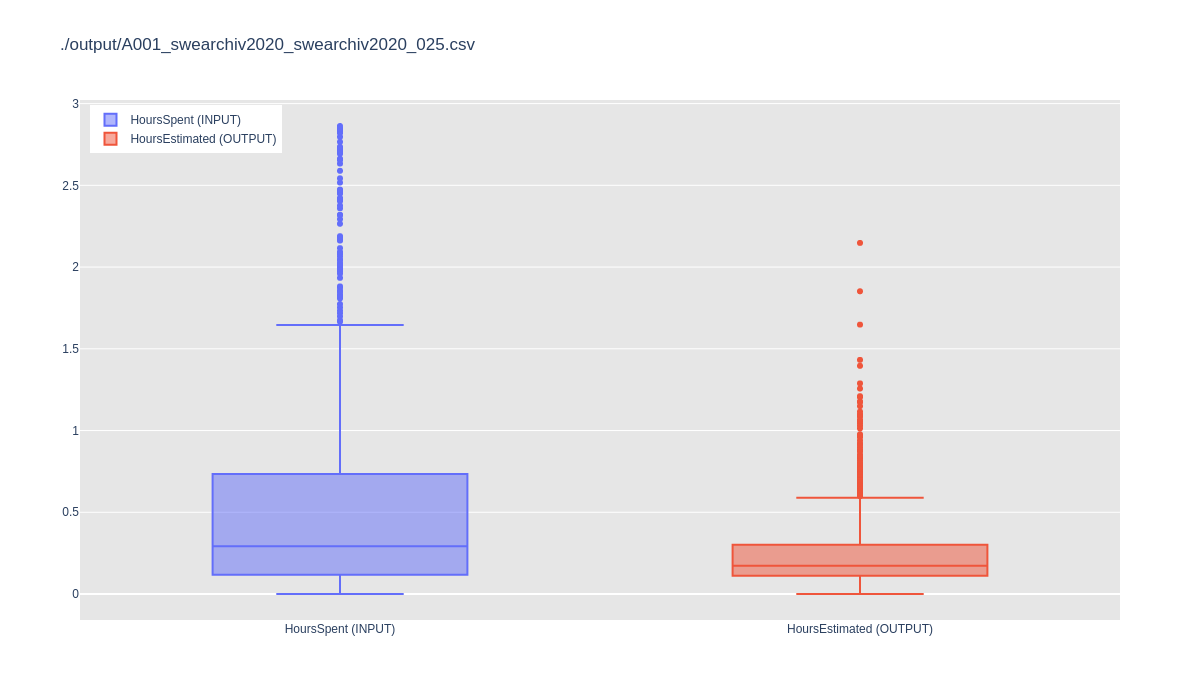
\includegraphics[width=\textwidth]{Scripts/output/A001_swearchiv2020_swearchiv2020_025.csv.png}
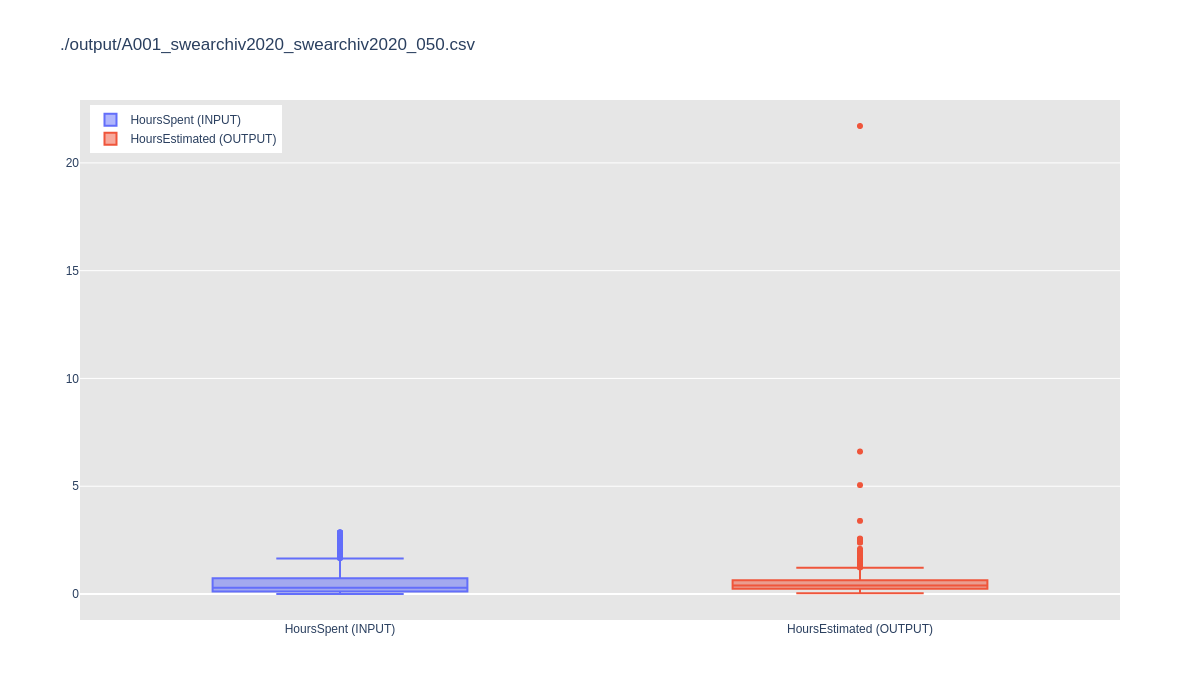
\includegraphics[width=\textwidth]{Scripts/output/A001_swearchiv2020_swearchiv2020_050.csv.png}
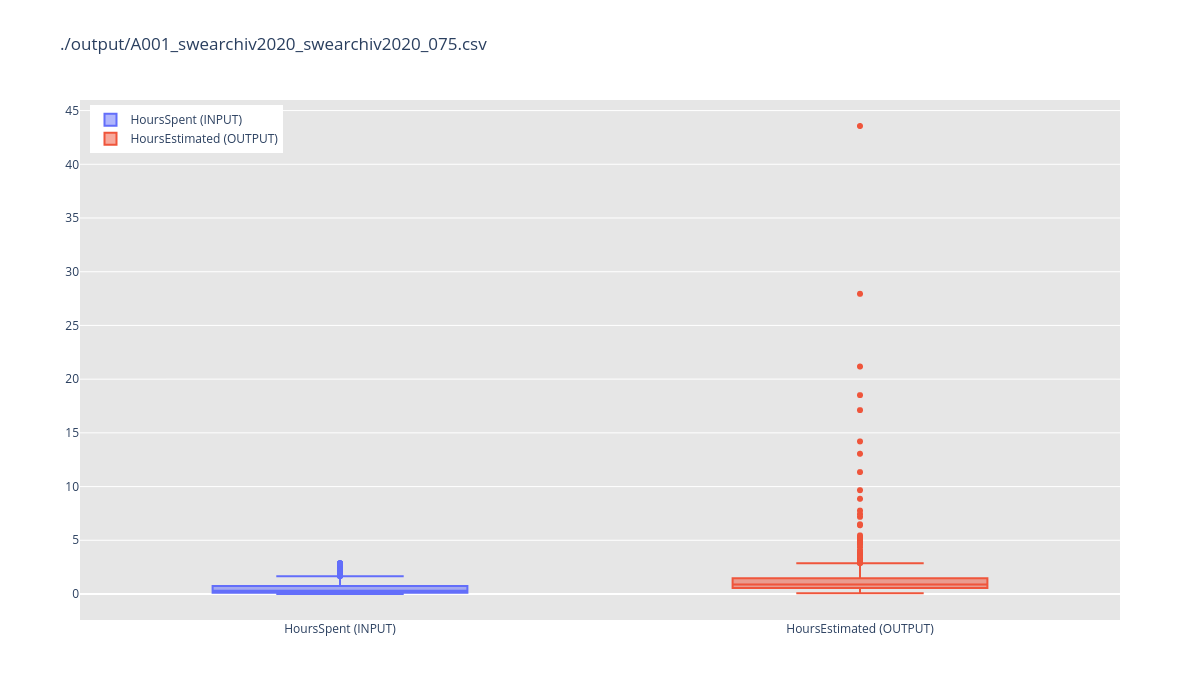
\includegraphics[width=\textwidth]{Scripts/output/A001_swearchiv2020_swearchiv2020_075.csv.png}
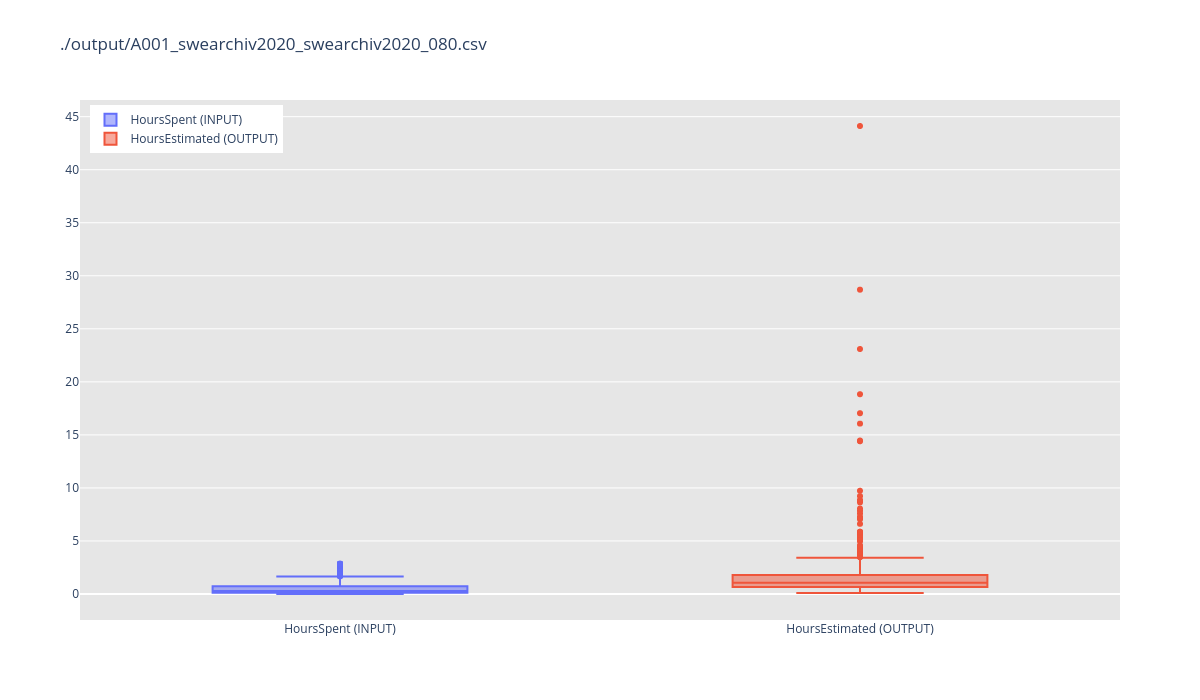
\includegraphics[width=\textwidth]{Scripts/output/A001_swearchiv2020_swearchiv2020_080.csv.png}
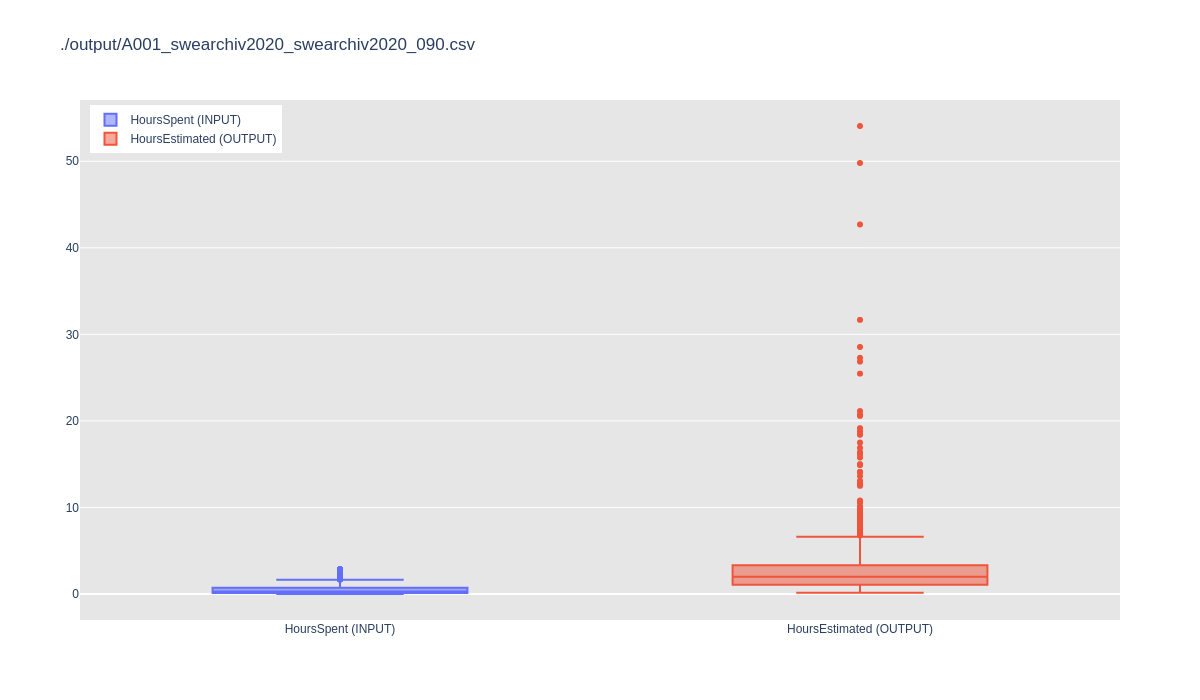
\includegraphics[width=\textwidth]{Scripts/output/A001_swearchiv2020_swearchiv2020_090.csv.png}
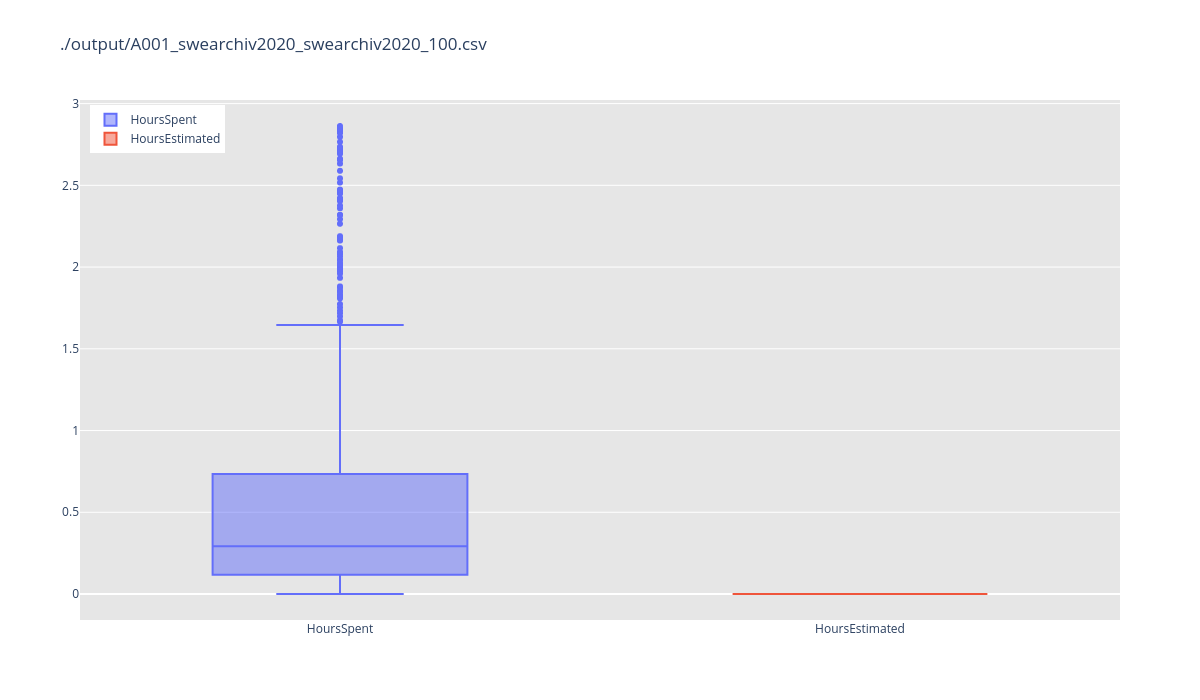
\includegraphics[width=\textwidth]{Scripts/output/A001_swearchiv2020_swearchiv2020_100.csv.png}
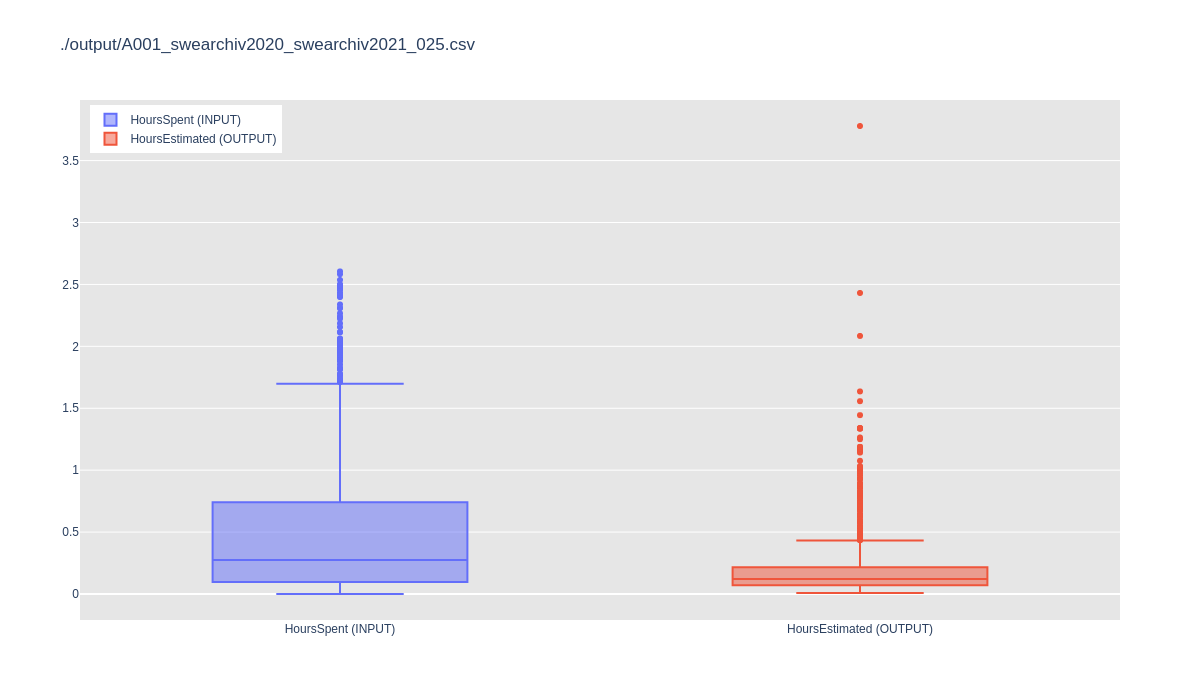
\includegraphics[width=\textwidth]{Scripts/output/A001_swearchiv2020_swearchiv2021_025.csv.png}
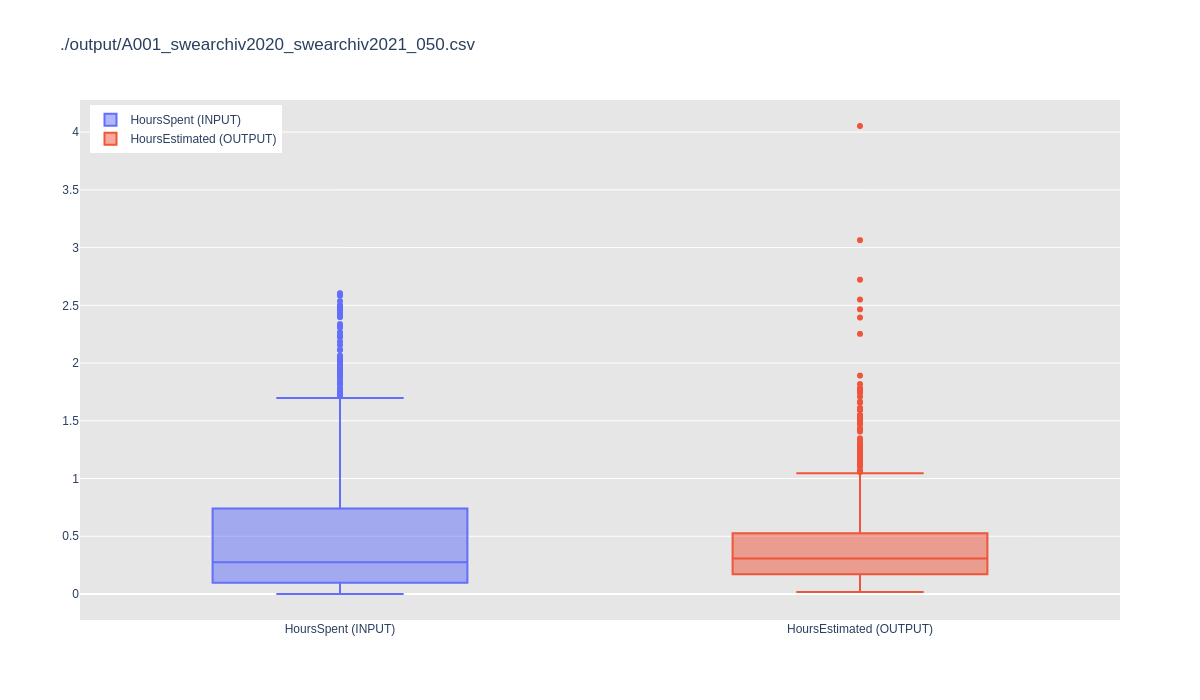
\includegraphics[width=\textwidth]{Scripts/output/A001_swearchiv2020_swearchiv2021_050.csv.png}
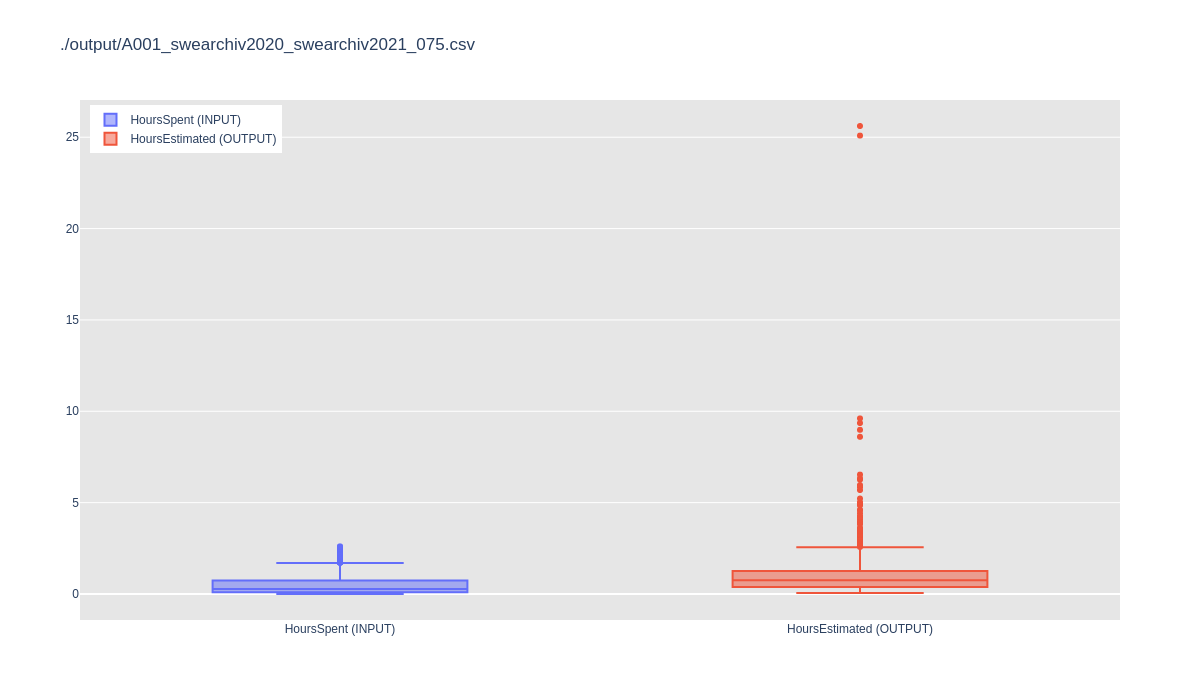
\includegraphics[width=\textwidth]{Scripts/output/A001_swearchiv2020_swearchiv2021_075.csv.png}
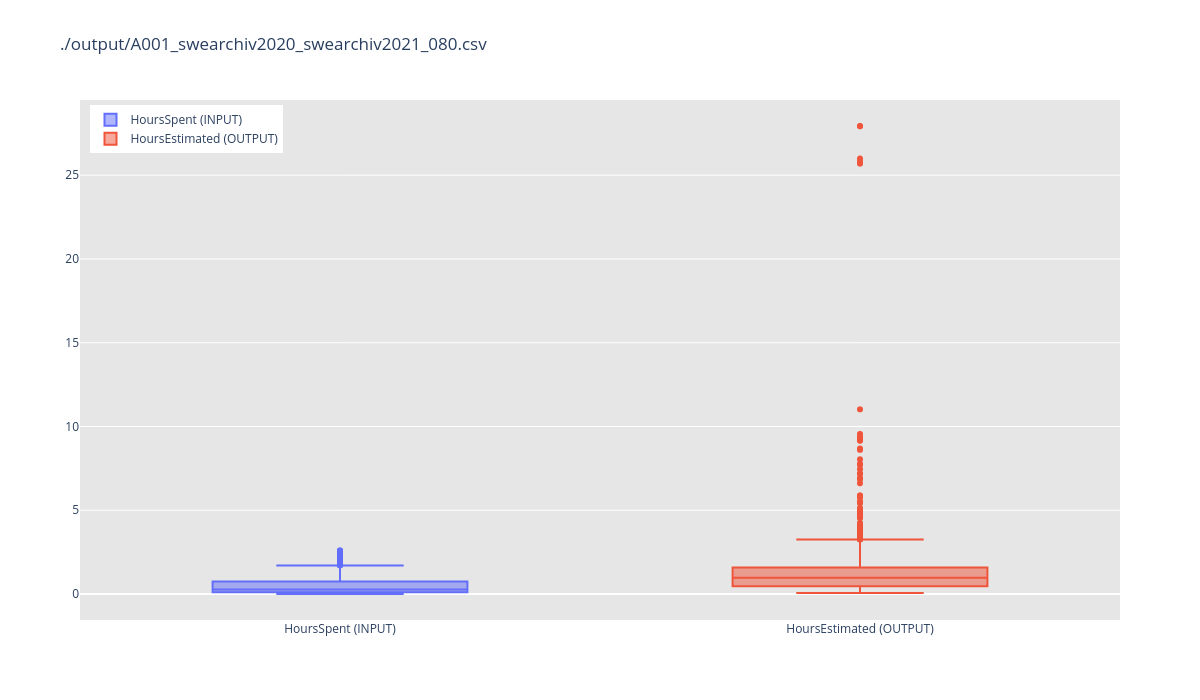
\includegraphics[width=\textwidth]{Scripts/output/A001_swearchiv2020_swearchiv2021_080.csv.png}
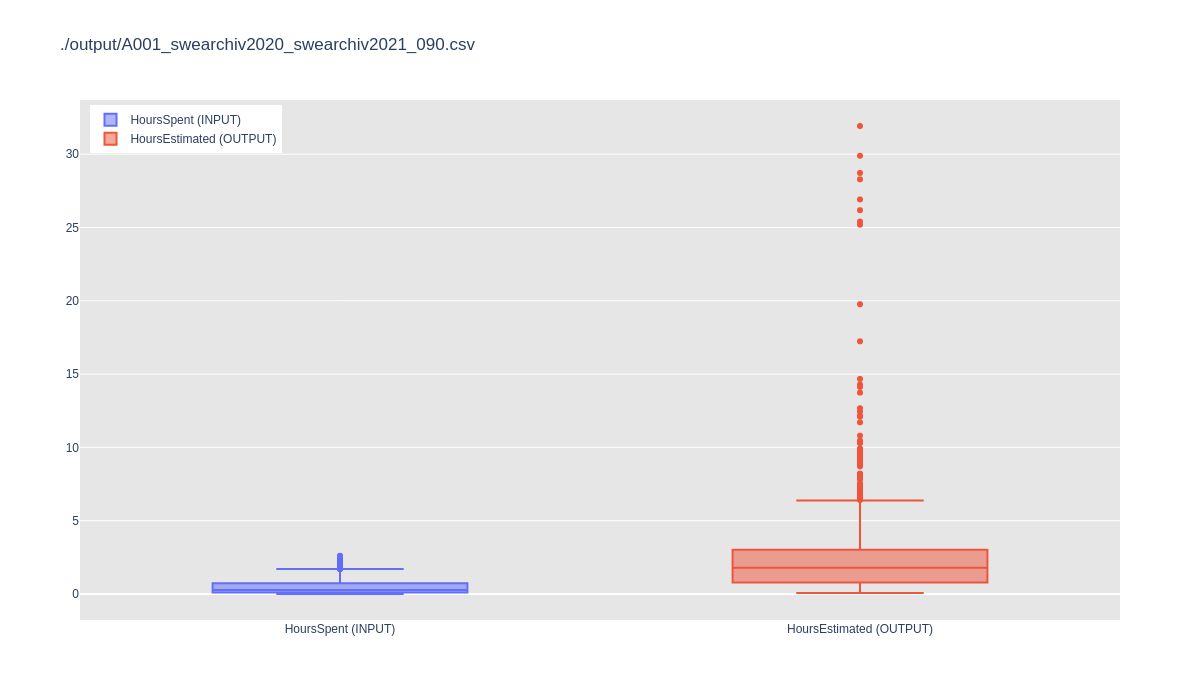
\includegraphics[width=\textwidth]{Scripts/output/A001_swearchiv2020_swearchiv2021_090.csv.png}
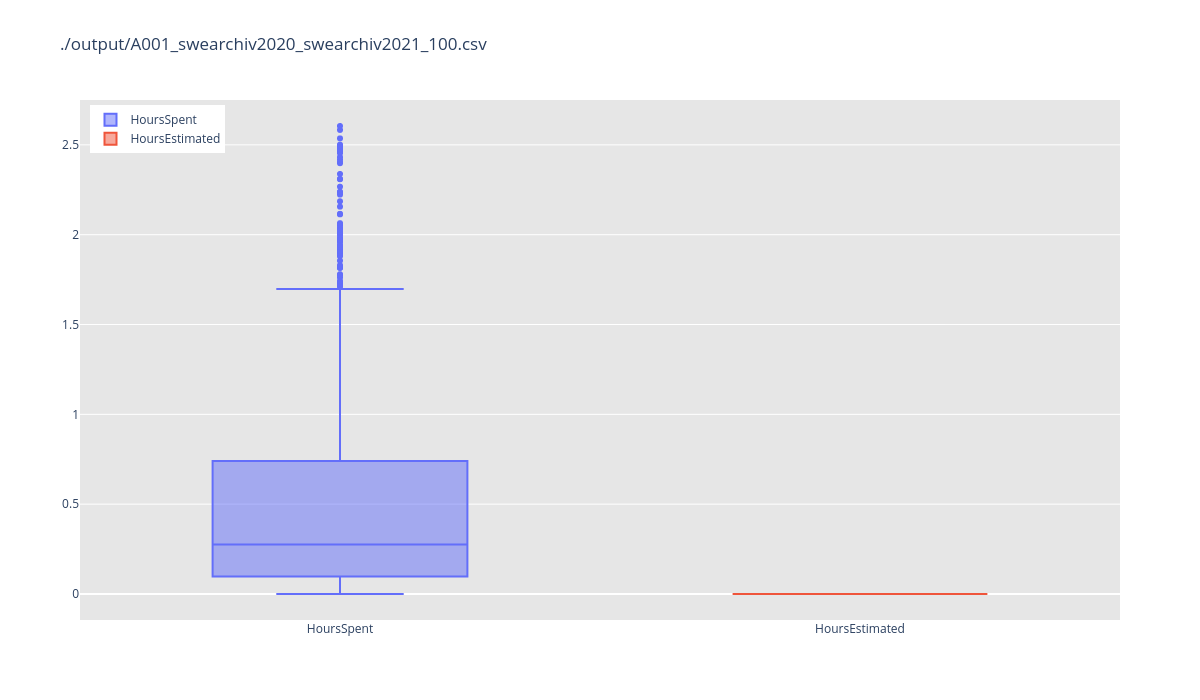
\includegraphics[width=\textwidth]{Scripts/output/A001_swearchiv2020_swearchiv2021_100.csv.png}




\end{document}

